\subsection{Komponenty wizualne}

Biblioteka {\bf System.Windows.Forms} udostępnia szereg gotowych komponentów. Wszystkie właściwości
obiektów są odpowiednimi składowymi klas opisujących te obiekty. Oprócz typowych składowych, przynależnych
wszystkim obiektom dziedziczącym w klasy {\bf Control}, każdy komponent ma szereg własnych, jemu tylko
właściwych składowych. Na przykład pole tekstowe ma właściwość {\bf MaxLength}, pozwalającą ustalić maksymalną
długość wprowadzanego napisu, czy propercję {\bf AcceptsEnter}, decydującą o tym, czy naciśnięcie klawisza
Enter w obrębie pola tekstowego dołączy do wprowadzanego tekstu znak przejścia do nowej linii, czy też
spowoduje przejście do kolejnego komponentu w oknie.

\subsubsection{ComboBox, ListBox}

Oba komponenty, {\bf ComboBox} i {\bf ListBox}, mają bardzo podobne zastosowanie i bardzo podobny interfejs
służący do oprogramowywania ich. Udostępniają one kolekcję
{\bf Items}, która przechowuje elementy pokazywane na listach tych komponentów. W najprostszym scenariuszu
napisalibyśmy po prostu:

\begin{scriptsize}
\begin{verbatim}
...
ComboBox cbItems;
...
cbItems.Add( "napis 1" );
cbItems.Add( "napis 2" );
cbItems.Add( "napis 3" );
...
\end{verbatim}
\end{scriptsize}

Pojawia się jednak pytanie: w jaki sposób aplikacja może być poinformowana o wyborze konkretnego
elementu przez użytkownika? Przypomnijmy sobie, że na poziomie Win32API z każdym elementem {\bf ComboBoxa} można
skojarzyć 32-bitową wartość, która może służyć do identyfikowania elementów (może na przykład przechowywać
identyfikator bazodanowy elementu na liście)\footnote{Wartość tą można ustalić bądź pobrać za pomocą par 
komunikatów {\bf CB\_SETITEMDATA}, {\bf CB\_GETITEMDATA} oraz {\bf LB\_SETITEMDATA}, {\bf LB\_GETITEMDATA}.}.

W bibliotece okienkowej .NET elementami ComboBoxa i ListBoxa mogą być dowolne obiekty, nie tylko napisy.
Jeśli do listy zostaje dodany obiekt innego typu niż {\bf string}, na liście pojawia się jego reprezentacja
napisowa, zaś na liście zapamiętana jest referencja do obiektu. 

Aby zasymulować możliwość jaką daje Win32API, czyli umieszczanie na liście napisów i kojarzenie z każdym z nich
wartości 32-bitowej, można posłużyć się pomocniczą klasą, która będzie przechowywać pary: napis i wartość 32-bitową.
Zauważmy jednak, że programista nie jest ograniczony do jednej wartości skojarzonej z napisem, ponieważ
jest to tylko i wyłącznie kwestią zaprojektowania odpowiedniej klasy.

\begin{scriptsize}
\begin{verbatim}
/* Wiktor Zychla, 2003 */
using System;
using System.Windows.Forms;

namespace Example
{
  public class MyComboBoxItem
  {
    string text;
    int    id;

    public string Text
    {
      get { return text; }
    }

    public int ID
    {
      get { return id; }
    }

    public MyComboBoxItem( string text, int id )
    {
      this.text = text;
      this.id   = id;
    }
   
    public override string ToString()
    {
      return text;
    }  
  }

  public class CMainForm : Form
  {   
    ComboBox cbItems;

    public CMainForm()
    {
      cbItems = new ComboBox();
      cbItems.Items.Add( new MyComboBoxItem( "ala",  17 ) );
      cbItems.Items.Add( new MyComboBoxItem( "ma",   24 ) );
      cbItems.Items.Add( new MyComboBoxItem( "kota", 19 ) );
      cbItems.Items.Add( new MyComboBoxItem( "!",    78 ) );
      cbItems.SelectedIndexChanged += 
        new EventHandler( cbItems_SelectedIndexChanged );

      this.Controls.Add( cbItems );
    } 

    void cbItems_SelectedIndexChanged( object sender, EventArgs e )
    {
      if ( cbItems.SelectedItem != null )
      {
        MyComboBoxItem myItem = cbItems.SelectedItem as MyComboBoxItem;
        MessageBox.Show( String.Format( "Wybrano element: {0} - {1}",
                            myItem.Text, myItem.ID ) );
      }
    }

    public static void Main()
    {
      Application.Run( new CMainForm() );
    }
  }
}
\end{verbatim}
\end{scriptsize}

\subsubsection{ToolTip}

Wyświetlaniem podpowiedzi zajmuje się obiekt typu {\bf ToolTip}. Podpowiedzi mogą składać się
z kilku linii tekstu. 

\begin{scriptsize}
\begin{verbatim}
/* Wiktor Zychla, 2003 */
using System;
using System.Drawing;
using System.Windows.Forms;

namespace Example
{
  public class CMainForm : Form
  {   
    Button b; 

    public CMainForm()
    {
      b = new Button();
      b.Text = "Kliknij mnie";
      this.Controls.Add( b );

      ToolTip tTip = new ToolTip();
      tTip.SetToolTip( b, "Podpowiedź\r\nwielolinijkowa" );
    } 

    public static void Main()
    {
      Application.Run( new CMainForm() );
    }
  }
}
\end{verbatim}
\end{scriptsize}

\subsubsection{ListView}

Komponent {\bf ListView} jest bardzo przydatny i w związku z tym często wykorzystywany w aplikacjach
Windowsowych. Potrafi pokazywać elementy w 4 różnych widokach\footnote{Cztery możliwości prezentowania
elementów listy przez {\bf ListView} najszybciej można zobaczyć w Eksplorerze Windows, który do pokazywania
elementów systemu plików używa właśnie ListView i pozwala przełączać się pomiędzy wszystkimi dostępnymi
widokami.}. Najczęściej korzysta się z widoku szczegółowego, w którym ListView staje się wielokolumnową listą
elementów. 

Inaczej niż w przypadku {\bf ComboBoxa}, elementy ListView są typu {\bf ListViewItem}. Jeżeli programista
chce skojarzyć własną informację z elementem listy, powinien skorzystać z propercji {\bf Tag} elementu, 
która może przechować referencję na dowolny obiekt. Również inaczej niż w przypadku {\bf ComboBoxa}, każdy
element ListView może mieć własny kolor tła i tekstu.

ListView wyróżnia się spośród innych komponentów tym, że potrafi samodzielnie sortować swoje elementy.
Wymaga to zdefiniowania klasy implementującej interfejs {\bf IComparer} i przypisania obiektu tej klasy do
propercji {\bf ListViewItemSorter} komponentu ListView.

\begin{figure}
\begin{center}
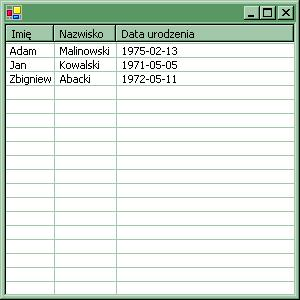
\includegraphics[width=0.50\textwidth]{./pic/swf03}
\caption{ListView potrafi sam sortować elementy umieszczone na liście}
\end{center}
\end{figure}

\begin{scriptsize}
\begin{verbatim}
/* Wiktor Zychla, 2003 */
using System;
using System.Collections;
using System.Drawing;
using System.Windows.Forms;

namespace Example
{
  // klasa do porównywania elementów ListView
  // wg. wskazanej kolumny
  public class MyLVItemSorter : IComparer
  {
    int kolumna; // kolumna wg. której sortujemy

    public MyLVItemSorter( int kolumna )
    {
      this.kolumna = kolumna;
    }

    public int Compare( object o1, object o2 )
    {
      ListViewItem l1 = o1 as ListViewItem;
      ListViewItem l2 = o2 as ListViewItem;

      return string.Compare( l1.SubItems[ kolumna ].Text,
                             l2.SubItems[ kolumna ].Text );
    }
  }

  public class CMainForm : Form
  {   
    ListView lstItems;

    void InitListViewElements()
    {
      string[] sHeaders = new string[] { "Imię", "Nazwisko", "Data urodzenia" };
      ListViewItem li;
     
      // nagłówki 
      lstItems.Columns.Clear();
      foreach ( string s in sHeaders )
        lstItems.Columns.Add( s, 60, HorizontalAlignment.Left ); 
      
      // elementy
      li = lstItems.Items.Add( "Jan" );     
      li.SubItems.Add( "Kowalski" );
      li.SubItems.Add( "1971-05-05" );

      li = lstItems.Items.Add( "Adam" );
      li.SubItems.Add( "Malinowski" );
      li.SubItems.Add( "1975-02-13" );

      li = lstItems.Items.Add( "Zbigniew" );
      li.SubItems.Add( "Abacki" );
      li.SubItems.Add( "1972-05-11" );

      // dopasuj szerokości kolumn
      foreach ( ColumnHeader ch in lstItems.Columns )
        ch.Width = -2;
    }

    // po kliku w kolumnę ListView ustal sortowanie wg. tej kolumny
    void LV_ColumnClick( object sender, ColumnClickEventArgs e )
    {
      lstItems.ListViewItemSorter = new MyLVItemSorter( e.Column );
    }

    public CMainForm()
    {
      lstItems      = new ListView();
      lstItems.Dock = DockStyle.Fill;
      lstItems.FullRowSelect = true;
      lstItems.GridLines = true;
      lstItems.View      = System.Windows.Forms.View.Details;       
      lstItems.ColumnClick += new ColumnClickEventHandler( LV_ColumnClick );
     
      this.Controls.Add( lstItems );

      InitListViewElements(); 
    } 

    public static void Main()
    {
      Application.Run( new CMainForm() );
    }
  }
}
\end{verbatim}
\end{scriptsize}

\subsubsection{TreeView}

Komponent {\bf TreeView} zyskał nowy, obiektowy interfejs, w którym każdy węzeł ma kolekcję {\bf Nodes}, 
przechowującą jego podwęzły. 

Z komponentem tym wiąże się klasyczny problem: jak radzić sobie z wypełnianiem struktury TreeView, jeśli 
powinien on przechowywać bardzo dużo danych? Oczywiście zainicjowanie całego drzewa w konstruktorze
okna macierzystego może nie wchodzić w grę, właśnie z powodu dużej ilości danych.

Problem ten rozwiązuje się zwykle tak, że inicjuje się tylko {\em jeden} poziom drzewa, poziom główny,
dodając przy okazji tym węzłom, które mają przechowywać jakieś podwęzły, tylko {\em jeden}, bardzo specjalny
"pusty" podwęzeł, oznaczony w propercji {\bf Tag} w jakiś określony sposób.

Następnie należy dodać funkcję obsługi zdarzenia {\bf BeforeExpand}, które pojawia się, gdy użytkownik
próbuje "rozwijać" węzeł drzewa przy pomocy symbolu "+" umieszczonego przy węźle. Wewnątrz funkcji obsługi
zdarzenia należy sprawdzić, czy rozwijany węzeł ma tylko jeden podwęzeł i to w dodatku ten specjalnie oznakowany.
Jeśli tak - należy ten podwęzeł usunąć i dobudować kolejny poziom drzewa, znów dodając specjalne
"puste" podwęzły określonym węzłom.

W ten sposób drzewo budowane jest zawsze "na życzenie", przy czym dobudowywany jest zawsze tylko ten poziom
drzewa, który jest akurat potrzebny.

\begin{figure}
\begin{center}
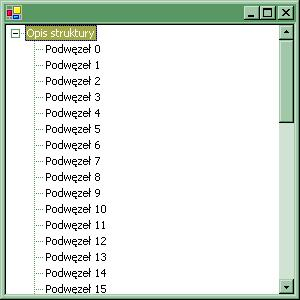
\includegraphics[width=0.50\textwidth]{./pic/swf04}
\caption{TreeView pozwala pokazać zależności między obiektami}
\end{center}
\end{figure}

\begin{scriptsize}
\begin{verbatim}
/* Wiktor Zychla, 2003 */
using System;
using System.Collections;
using System.Drawing;
using System.Windows.Forms;

namespace Example
{
  public class CMainForm : Form
  {   
    TreeView tvItems;

    void InitTVElements()
    {
      TreeNode treeRoot  = new TreeNode( "Opis struktury" );
      treeRoot.ForeColor = Color.Blue;

      TreeNode treeSubNode;
      for ( int i=0; i<45; i++ )
      {
        treeSubNode = new TreeNode( String.Format( "Podwęzeł {0}", i ) );
        treeRoot.Nodes.Add( treeSubNode );
      }   

      tvItems.Nodes.Add( treeRoot );
    } 

    public CMainForm()
    {
      tvItems      = new TreeView();
      tvItems.Dock = DockStyle.Fill;
     
      this.Controls.Add( tvItems );

      InitTVElements();
    } 

    public static void Main()
    {
      Application.Run( new CMainForm() );
    }
  }
}
\end{verbatim}
\end{scriptsize}

\subsection{Rozmieszczanie okien potomnych}

Dobrze zaprojektowany interfejs użytkownika powinien być czytelny i przejrzysty. Jednak przy odrobinie
wprawy i doświadczenia można sobie z tym poradzić. O wiele trudniej jest zaprojektować interfejs tak, aby
pozostawał spójny gdy okno zmienia swoje rozmiary, na przykład gdy jest rozciągane przez użytkownika.

Istnieją dwa możliwe rozwiązania: można albo zabronić zmian rozmiaru okna (przez ustawienie
propercji {\bf FormBorderStyle} na {\bf FormBorderStyle.FixedDialog}) albo reagować na zmianę rozmiaru
okna i dopasowywać rozmiary okien potomnych do rozmiaru okna macierzystego. Oczywiście nie zawsze można
po prostu zabronić zmian rozmiaru okna. Czy w związku z tym .NET wspomaga jakoś proces rozmieszczania
okien potomnych przy zmianie rozmiaru okna macierzystego? Otóż tak. 

\subsubsection{Kotwice i dokowanie}

Najprostszy sposób dopasowywania rozmiarów okna potomnego do rozmiarów okna 
macierzystego to tzw. {\em kotwicowanie}. Wystarczy nadać oknu potomnemu właściwość 
{\em bycia zaczepionym} któregoś z boków okna macierzystego, aby okno potomne zachowywało odległość
od odpowiedniego boku podczas zmiany rozmiarów okna macierzystego.

\begin{scriptsize}
\begin{verbatim}
/* Wiktor Zychla, 2003 */
using System;
using System.Drawing;
using System.Windows.Forms;

namespace Example
{
  public class CMainForm : Form
  {   
    Button b; 

    public CMainForm()
    {
      b          = new Button();
      b.Text     = "Kliknij mnie";
      b.Location = new Point( 40, 40 );
      b.Anchor   = AnchorStyles.Bottom |
                   AnchorStyles.Top    |
                   AnchorStyles.Left   |
                   AnchorStyles.Right;

      this.Controls.Add( b );
    } 

    public static void Main()
    {
      Application.Run( new CMainForm() );
    }
  }
}
\end{verbatim}
\end{scriptsize}

\begin{figure}
\begin{center}
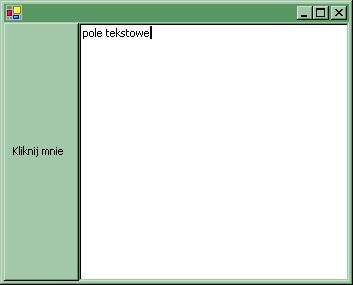
\includegraphics[width=0.50\textwidth]{./pic/swf02}
\caption{Okna potomne zadokowane w obrębie okna macierzystego}
\end{center}
\end{figure}

Okna potomne można również {\em dokować}, czyli przywiązywać na stałe do któregoś z boków lub całego obszaru 
okna macierzystego. Dokowanie jest szczególnie przydatne w przypadku dwóch okien potomnych, bowiem jedno z nich
można zadokować do któregoś z boków, a drugie do całego obszaru okna. Oba okna potomne zajmą wtedy
cały obszar okna macierzystego i będą poprawnie dostosowywać się do zmian jego rozmiaru.

Należy jedynie pamiętać o tym, aby to okno potomne, które powinno wypełniać obszar okna macierzystego
było umieszczone "na wierzchu", czyli nad oknem zadokowanym do któregoś z boków. 

\begin{scriptsize}
\begin{verbatim}
/* Wiktor Zychla, 2003 */
using System;
using System.Drawing;
using System.Windows.Forms;

namespace Example
{
  public class CMainForm : Form
  {   
    Button  b; 
    TextBox t;

    public CMainForm()
    {
      b           = new Button();
      b.Text      = "Kliknij mnie";
      b.Dock      = DockStyle.Left;

      t           = new TextBox();
      t.Multiline = true; 
      t.Dock      = DockStyle.Fill;
      
      this.Controls.Add( t );
      this.Controls.Add( b );
    } 

    public static void Main()
    {
      Application.Run( new CMainForm() );
    }
  }
}
\end{verbatim}
\end{scriptsize}

\subsubsection{Panele}

Sytuacja, w której okno macierzyste ma tylko dwa okna potomne jest niezwykle rzadka. Zastosowanie
pokazanej powyżej metody wydaje się być więc dość ograniczone. Okazuje się jednak, że istnieje specjalny typ
komponentu, {\bf Panel}, który z jednej strony zachowuje się jak okno potomne, bowiem jest 
komponentem umieszczanym wewnątrz jakiegoś okna dialogowego, z drugiej strony zachowuje się jak
okno macierzyste, bowiem ma swoją własną kolekcję okien potomnych, które są kotwicowane i dokowane 
względem obszaru Panela, a nie okna macierzystego.

Można więc używać paneli do podziału okna macierzystego na drobniejsze fragmenty, w obrębie których można
dokonywać odpowiednich ustaleń rozmieszczenia okien potomnych. Panele można zagnieżdżać.

\begin{scriptsize}
\begin{verbatim}
/* Wiktor Zychla, 2003 */
using System;
using System.Drawing;
using System.Windows.Forms;

namespace Example
{
  public class CMainForm : Form
  {   
    Panel   p;
    Button  b1; 
    Button  b2; 
    TextBox t;

    public CMainForm()
    {
      // panel zadokowany do lewej, a w nim dwa przyciski
      p           = new Panel();
      p.Dock      = DockStyle.Left;      

      b1          = new Button();
      b1.Text     = "Kliknij mnie";
      b1.Dock     = DockStyle.Top;

      b2          = new Button();
      b2.Text     = "Kliknij mnie";
      b2.Dock     = DockStyle.Fill;
      
      p.Controls.Add( b2 );
      p.Controls.Add( b1 );

      // pole tekstowe wypełnia obszar okna
      t           = new TextBox();
      t.Multiline = true; 
      t.Dock      = DockStyle.Fill;

      this.Controls.Add( t );
      this.Controls.Add( p );
    } 

    public static void Main()
    {
      Application.Run( new CMainForm() );
    }
  }
}
\end{verbatim}
\end{scriptsize}

\subsubsection{Splittery}

Splittery są elementami graficznymi w postaci poziomych lub pionowych "belek", pozwalających
użytkownikowi zmienić rozmiary okien potomnych. Splitterów używa się tam, gdzie używa się dokowania.

\begin{scriptsize}
\begin{verbatim}
/* Wiktor Zychla, 2003 */
using System;
using System.Drawing;
using System.Windows.Forms;

namespace Example
{
  public class CMainForm : Form
  {   
    Panel   p;   // zawiera b1 i b2  
    Button  b1; 
    Button  b2; 
    TextBox t;

    Splitter s1; // rozdziela b1 i b2
    Splitter s2; // rozdziela p  i t

    public CMainForm()
    {
      // panel zadokowany do lewej, a w nim dwa przyciski
      p           = new Panel();
      p.Dock      = DockStyle.Left;      

      b1          = new Button();
      b1.Text     = "Kliknij mnie";
      b1.Dock     = DockStyle.Top;

      s1          = new Splitter();
      s1.Dock     = DockStyle.Top;

      b2          = new Button();
      b2.Text     = "Kliknij mnie";
      b2.Dock     = DockStyle.Fill;
      
      p.Controls.Add( b2 );
      p.Controls.Add( s1 ); // splitter rozdziela b2 i b1
      p.Controls.Add( b1 );

      // pole tekstowe wypełnia obszar okna
      s2          = new Splitter();
      s2.Dock     = DockStyle.Left;

      t           = new TextBox();
      t.Multiline = true; 
      t.Dock      = DockStyle.Fill;

      this.Controls.Add( t );
      this.Controls.Add( s2 ); // splitter rozdziela t i p
      this.Controls.Add( p );
    } 

    public static void Main()
    {
      Application.Run( new CMainForm() );
    }
  }
}
\end{verbatim}
\end{scriptsize}
